\documentclass[../main.tex]{subfiles}

% Importing images from another path
\graphicspath{{\subfix{../images/}}}

\begin{document}

As previously anticipated, scalability has been assessed for all the 
implemented algorithms and the results are presented in this section. All the
measurements have been conducted on the \textit{ORFEO} cluster of the AREA Science Park in Trieste, using a single node of the \textit{EPYC} partition. These nodes are equipped with 2 sockets, each of which has an AMD EPYC 7H12 (Rome) cpu installed, for a total of 128 cores~\cite{epyc}.\\
Strong scalability of all the algorithms has been tested by feeding the different implementation with an input array of fixed dimension and incrementally increasing the number of processes involvend. The input array to be sorted contained randomly generated numbers that are homogeneously distributed in the range $[0,1)$. For each possible value of processes and each algorithm, the sorting time has been collected multiple times on different input arrays\footnote{All having the same fixed size, but different randomly generated numbers.} in order to estimate average time and standard deviation.\\
On the other hand, weak scalability has been assessed by incrementally increasing the number of processes involved, but having an input array that guaranteed to have a fixed \textit{workload-per-process}. This has of course been achieved by generating at each run a number of elements proportional to the processes. Also in this case multiple sorting times for different inputs have been collected in order to have a significant statistical sample.\\
\begin{figure}[b]
    \centering
    \begin{minipage}{0.50\textwidth}
        \centering
        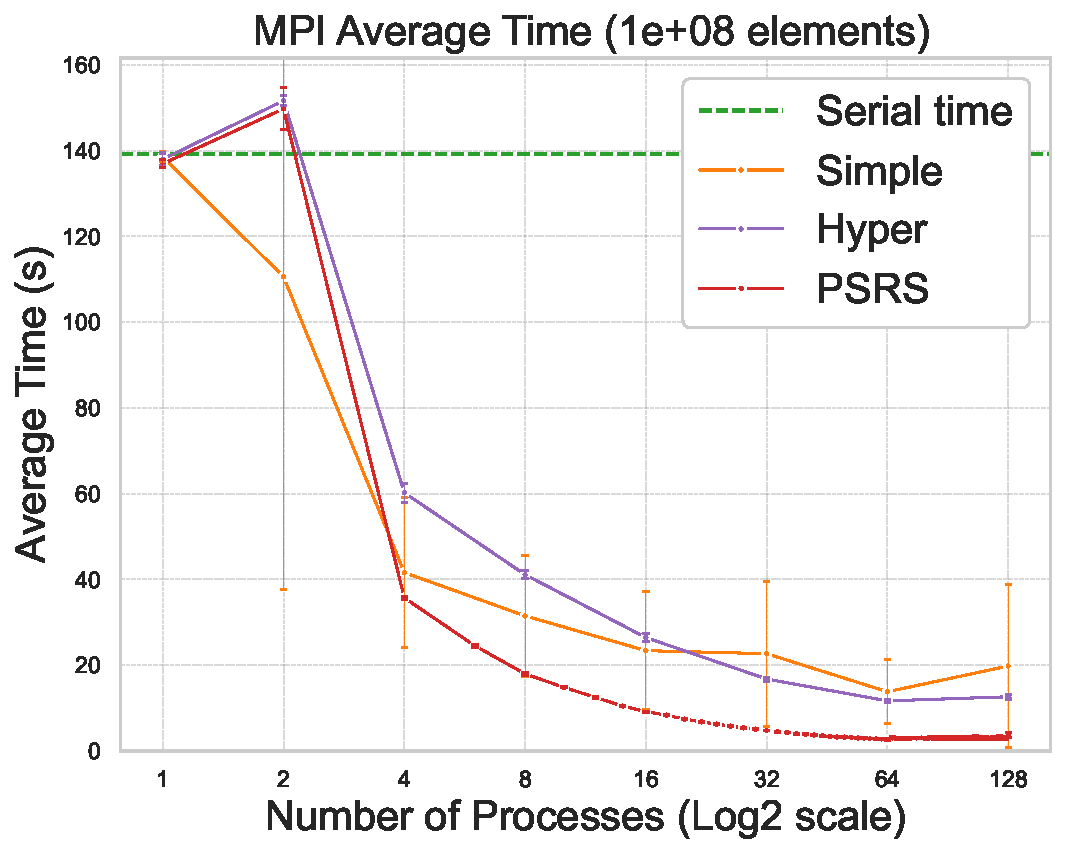
\includegraphics[width=1\textwidth]{mpi_timeplot.pdf}
    \end{minipage}\hfill
    \begin{minipage}{0.50\textwidth}
        \centering
        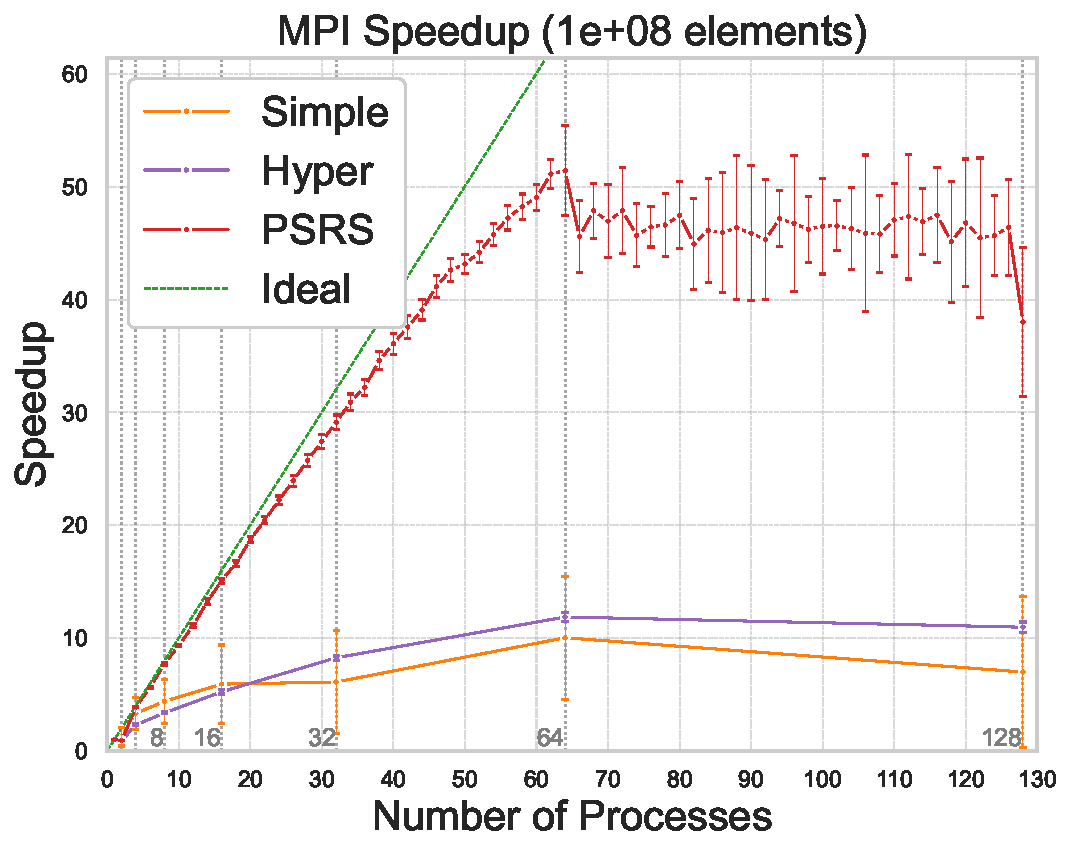
\includegraphics[width=1\textwidth]{mpi_speedplot.pdf}
    \end{minipage}

    \caption{Strong scalability of the MPI implementations. On the left, the average sorting time against the number of processes for $100$ million elements. On the right, the speedup against the number of processes. All results have been obtained with $2$ threads per core.}
    \label{fig:strong_mpi}
\end{figure}
Figure~\ref{fig:strong_mpi} summarizes the results obtained for the strong scalability test of the distributed memory algorithms implemented in MPI, for a fixed size array of $100$ million elements. As expected, the algorithm showing the best scalability results is indeed the \textbf{PSRS} algorithm. It's possible to see from the speedup plot that the algorithm scales almost linearly up to $64$ processes with great consistence and then it starts to slow down for higher numbers of processes by also increasing the variability of the results. Another noticeable aspect is that the \textbf{Hyperquicksort} algorithm shows improvements upon the \textbf{Simple Parallel Quicksort} only when the number of processes exceeds $16$. This is expected and can be explained with the fact that the overhead of the initial local sort in the former algorithm is compensated only by a large number of processes, that depends on the input size of the array. On the other hand however, the \textbf{Simple Parallel Quicksort}, although running faster for small numbers of processes, shows the largest variability among all the algorithms as highligted by the high values measured for the standard deviations in the different runs of the test. This is in agreement to the theoretical expectations, since the algorithm is highly dependent on the choice of the pivot and the initial distribution of the elements among the processes.\\
Similar results have been obtained for the weak scalability test where a fixed \textit{workload-per-process} of $1$ million elements has been used for all possible number of processes, as shown in 
figure~\ref{fig:weak_mpi}. All the algorithms perform significantly better than the serial version, with the \textbf{PSRS} algorithm showing the best results among the three. In particular, in the worst-case-scenario with $128$ processes, the \textbf{PSRS} performed $27$ times better than the serial equivalent\footnote{``Serial equivalent'' means the time of the serial implementation with $1$ process multiplied by $128$, the highest number of processes used in the parallel versions.}, while the other two implementations only performed $10$ times better. In terms of efficiency, the \textbf{PSRS} algorithm maintains an average above $70\%$ up to $64$ processes, while the efficiency of the other two algoritms struggle to remain above $50\%$ even for relatively small number of processes.\\
\begin{figure}[t]
    \centering
    \begin{minipage}{0.50\textwidth}
        \centering
        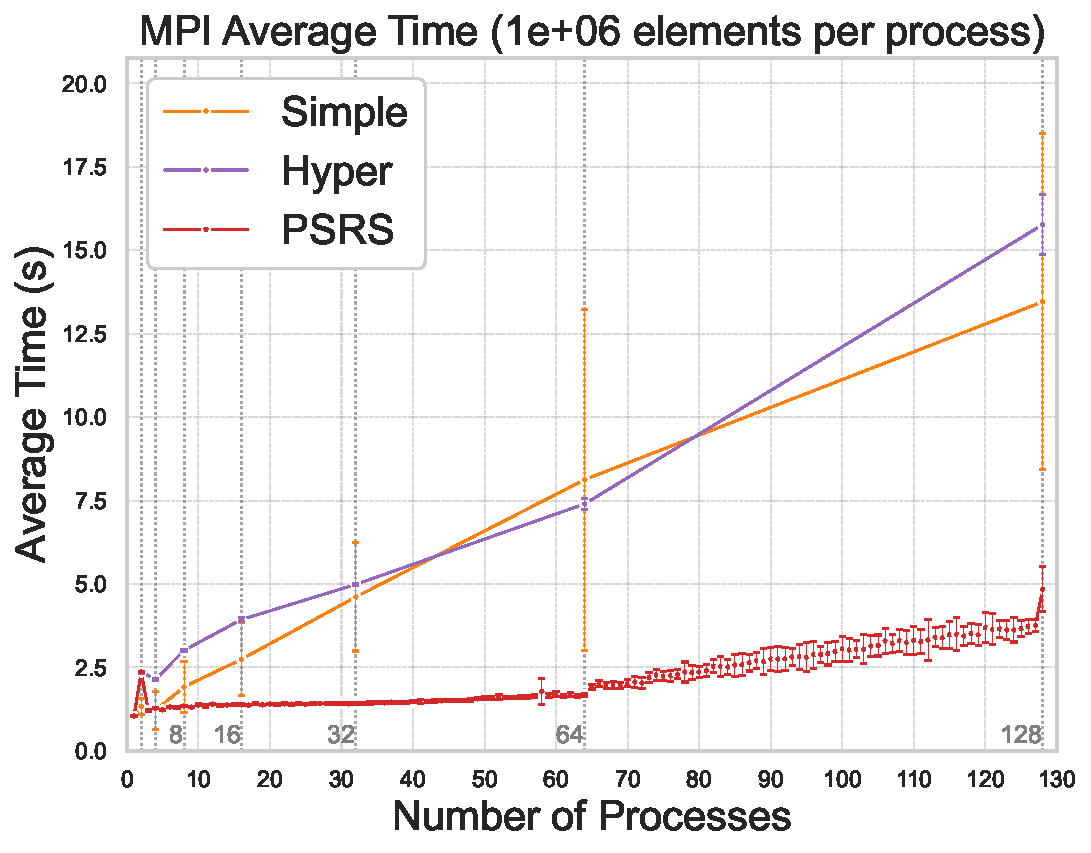
\includegraphics[width=1\textwidth]{mpi_weaktimeplot.pdf}
    \end{minipage}\hfill
    \begin{minipage}{0.50\textwidth}
        \centering
        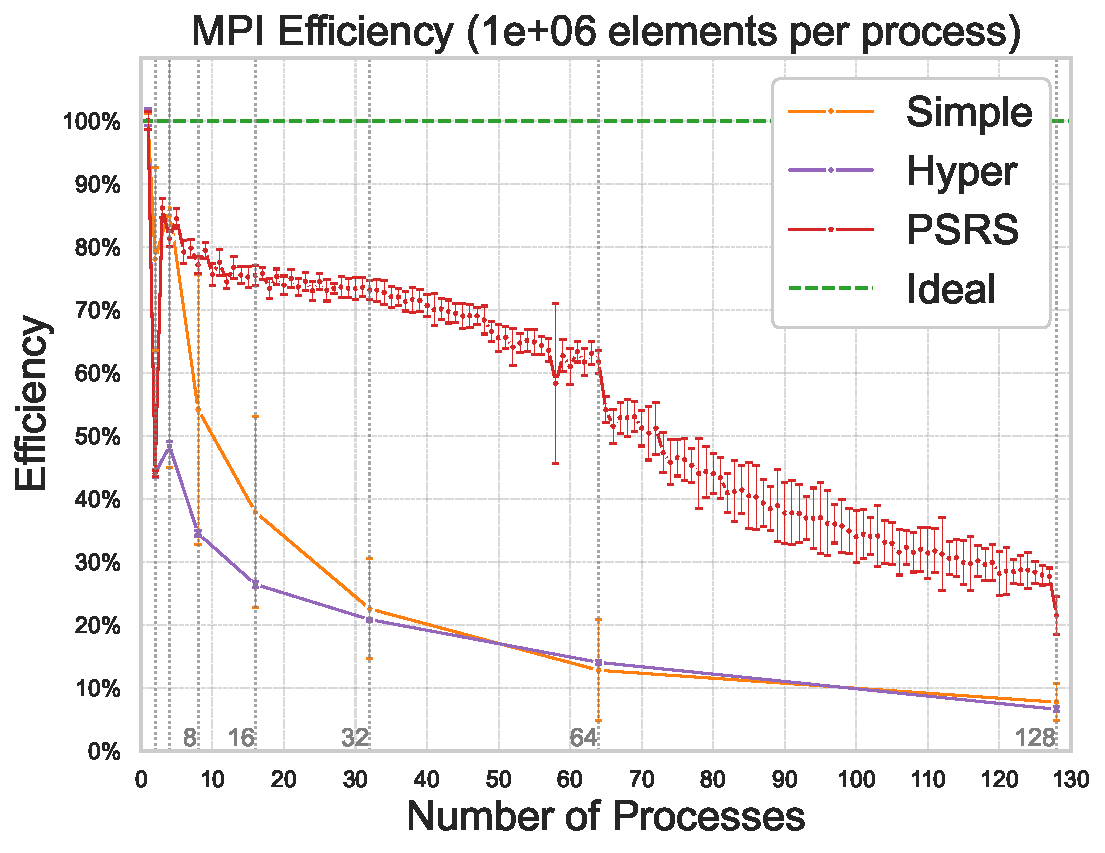
\includegraphics[width=1\textwidth]{mpi_effplot.pdf}
    \end{minipage}

    \caption{Weak scalability of the MPI implementations. On the left, the average time against the number of processes for $1$ million elements per process. On the right, the efficiency vs.\ the number of processes. All results have been obtained with $2$ threads per core.}
    \label{fig:weak_mpi}
\end{figure}
The strong scalability results obtained for the OpenMP algorithms are shown in figure~\ref{fig:strong_omp}. The input array used for this test contained $10$ million elements and the number of threads has been increased up to $64$ for each algorithm. The plots show that the best scaling algorithm among the different shared memory implementation is the task-based quicksort, which turns out to be the best alternative both in terms of perfomance and overall implmentation complexity. As highligted from the speedup plot, this algorithm show an initial linear speedup that then decreases after only $16$ threads. Noticeably, the \textbf{PSRS} algorithm shows good results even with its shared memory implementation. Although its speedup does not quite match the \textbf{Task Quicksort} nor the one of its distributed memory counterpart, it still constitutes a valid implementation up to $64$ threads when compared to the serial version. The results obtained with the \textbf{Simple Parallel Quicksort} and the \textbf{Hyperquicksort} shared memory implementations, on the other hand, turned out to be even worse than the serial version for increasing number of threads. As anticipated, this was partially expected due to the serial sorting that need to be carried out by a single thread before advancing to the next recursive call. Therefore, in these cases, the addition of new threads only increases the parallelization overhead of the multiple parallel regions and the need of further synchronization among larger number of threads without bringing any real benefit.\\
\begin{figure}[b]
    \centering
    \begin{minipage}{0.50\textwidth}
        \centering
        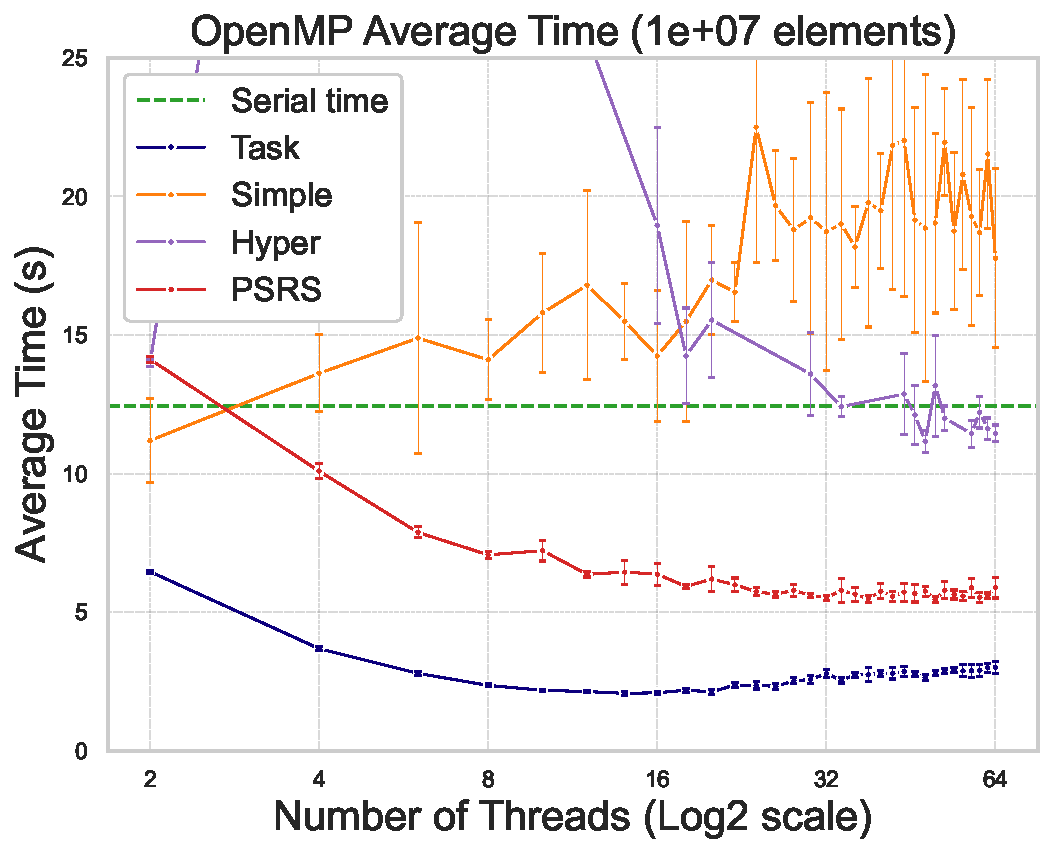
\includegraphics[width=1\textwidth]{omp_timeplot.pdf}
    \end{minipage}\hfill
    \begin{minipage}{0.50\textwidth}
        \centering
        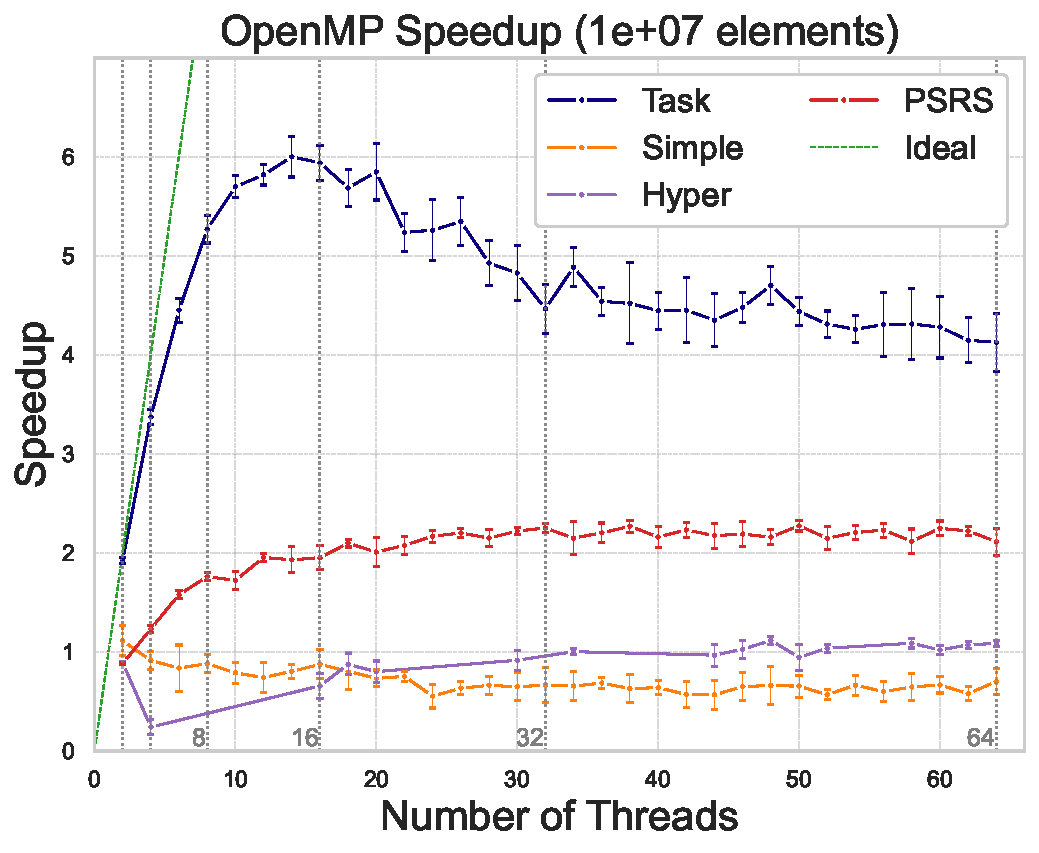
\includegraphics[width=1\textwidth]{omp_speedplot.pdf}
    \end{minipage}

    \caption{Strong scalability of the OpenMP implementations. On the left, the average sorting time against the number of threads for $10$ million elements. On the right, the speedup vs.\ the number of threads.}
    \label{fig:strong_omp}
\end{figure}
The weak scaling analysis has therefore been conducted only on the \textbf{Task Quicksort} and the \textbf{PSRS} algorithms, as shown in figure~\ref{fig:weak_omp}. The input array used for this test contained $1$ million elements per thread. The result of this test are similar to the ones previously presented, with the \textbf{Task Quicksort} having the most promising results among the two, showing an improvement on the serial version of a factor of $4$, while the shared version of the \textbf{PSRS} performed about $\sim 1.6$ times better than the serial equivalent with $64$ threads. Efficiency results in this case, however, are noticeably worse for both algorithms when compared to the distributed memory implementations: the \textbf{Task Quicksort} maintains an average efficiency of $50\%$ only up to $8$ cores, whereas the \textbf{PSRS} algorithm never shows efficiency above $50\%$ for any number of threads in the tested range.\\
\begin{figure}[t]
    \centering
    \begin{minipage}{0.50\textwidth}
        \centering
        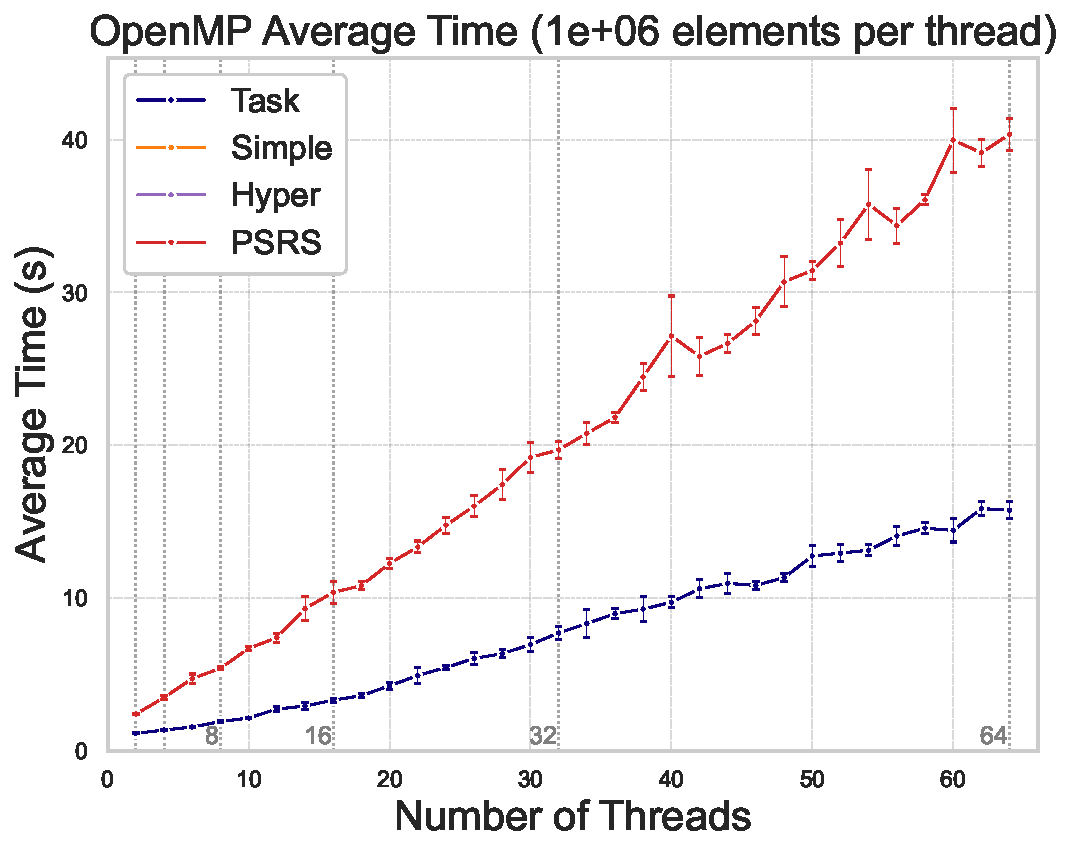
\includegraphics[width=1\textwidth]{omp_weaktimeplot.pdf}
    \end{minipage}\hfill
    \begin{minipage}{0.50\textwidth}
        \centering
        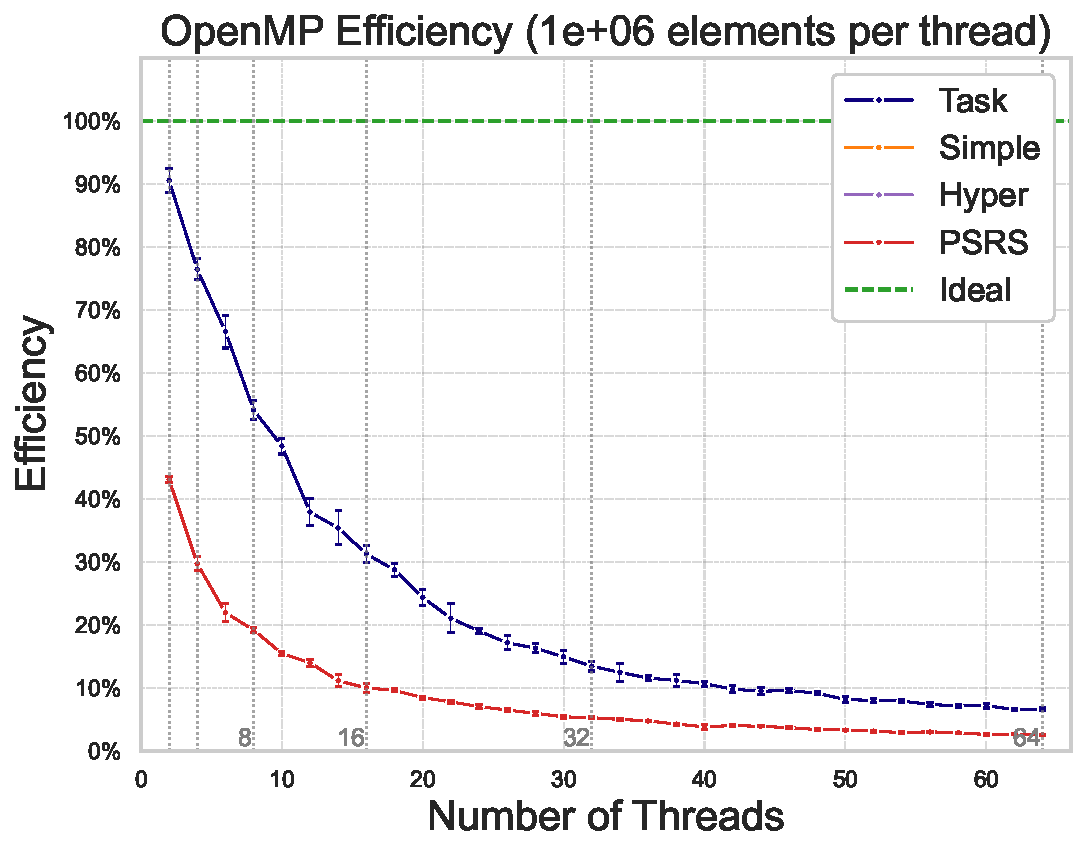
\includegraphics[width=1\textwidth]{omp_effplot.pdf}
    \end{minipage}

    \caption{Weak scalability of the OpenMP implementations. On the left, the average sorting time against the number of threads for $1$ million elements per thread. On the right, the efficiency vs.\ the number of threads.}
    \label{fig:weak_omp}
\end{figure}

\end{document}
